%
\tableofcontents
%


\section{Experiments: Supplementary Material}\label{sec:app:experiments-supplementary}

\subsection{Details on Experimental Setup}\label{sec:app:experiment-setup}

\paragraph{Datasets.} Below is a short description and source for the two main datasets we use in the analysis. Within each dataset, the sequence length is the same across runs ($2048$ for \li{}, and $4096$ for \oellm{}). For the scaling laws, we select for each combination of $(N,b,D)$ (model size, batch size, token budget) the learning rate that obtains smallest final loss.

%%%%%%%%%%%%%%%%%%%%%%%%%%%%%%%%%%%%%%%%%%%%%%%%%%%%%%%%%%%%%%%%%%%%%%%%%%%%
\noindent\rule{\textwidth}{1pt}
\begin{description}[listparindent=0pt,leftmargin=1.0em,]
	% Stepfun
	\item[\li] \hfill \citep{Li2025}~\\[.5em]
    %
	Training logs for different model sizes, token budgets, batch sizes, and learning rates. We use their smoothened loss and filter on dense models (no MoEs).
	
	%\vspace{1ex}
	
    \begin{tabular}{@{}ll@{}}
		Source & \small \url{https://wandb.ai/billzid/predictable-scale}
	\end{tabular}

    % OpenEuroLLM
	\item[\oellm] \hfill \citep{OpenEuroLLM2026}~\\[.5em]
    %
    This is an unpublished dataset of training runs executed by the \href{www.openeurollm.eu}{OpenEuroLLM initiative}. Additional details on the training setup will be provided upon its release 
	by the OpenEuroLLM initiative. 
	
	
\end{description}
\noindent\rule{\textwidth}{1pt}
%%%%%%%%%%%%%%%%%%%%%%%%%%%%%%%%%%%%%%%%%%%%%%%%%%%%%%%%%%%%%%%%%%%%%%%%%%%%


\begin{table}[H]
    \centering
    \caption{Overview of the datasets used for fitting our scaling laws. Here, we report the ranges of $(N,M,K)$ on the union of train and validation set. See also \cref{fig:data-overview-li}.}
    \begin{tabular}{|c|cc|}
        \hline
        \textbf{Name} & \li{} &  \oellm{} \\[1pt]
        \hline \hline
        Samples (train/val) & (246/54) & (191/21) \\
        Range of $N$ & $[59, 1073] ~(\cdot 10^6)$ & $[50, 1000]~(\cdot 10^6)$ \\
        Range of $M$ & $[0.032,4.2] ~(\cdot 10^6)$ & $[0.65,4.19] ~(\cdot 10^6)$ \\
        Range of $K$ & $[0.9, 1525] ~(\cdot 10^3)$ & $[7.1,1144.4] ~(\cdot 10^3)$ \\
        Range of $\mathcal{L}$ & $[2.12, 3.14]$ & $[2.08,2.93]$ \\
        \hline
    \end{tabular}
    \label{tab:dataset-overview}
\end{table}
%

\paragraph{Fitting methodology.} We first describe the procedure for fitting the scaling laws. The training set is split into five parts of equal size. For each law, we then fit the same law on each leave-one-out split of datapoints (five-fold cross-validation). This allows for more robustness to outliers and to quantify uncertainty for each fitted parameter.

For the fitting procedure, we use the same Huber loss function as \citet{Besiroglu2024}: for true loss values $\mathcal{L}_{\text{true}}$ and predicted loss values $\hat{\mathcal{L}}$, we minimize
\begin{align*}
    \sum_{i} \mathcal{H}_\delta\big(\log(\mathcal{L}^{(i)}_{\text{true}}) - \log(\hat{\mathcal{L}}^{(i)}\big), \quad 
    \mathcal{H}_\delta(z) = \begin{cases}
        \frac12 \delta^2, \quad &|z| \leq \delta, \\
        \delta(|z|-\frac12 \delta), \quad &\text{else}.
    \end{cases}
\end{align*}
We use the \texttt{minimize} method from \texttt{scipy.optimize} together with the \texttt{L-BFGS-B} optimizer.

\paragraph{Choice of $\delta$.} For the Huber loss, we set $\delta=10^{-3}$ for the \ttl{} and \tttl{} scaling laws, which is the standard value used also by \citet{Besiroglu2024}. We run an ablation on this choice, setting  $\delta =10^{-5}$ instead, see \cref{sec:app:ablation-delta} for details.

\paragraph{Initialization.} For each single fit, we minimize the Huber loss at $n_{\text{init}}$ different initializations  with \texttt{L-BFGS}, and select the solution that results in the smallest objective function. By default, we use a grid of ten values for each of $(\alpha, \beta, \gamma, E)$ and two values for each of $(A,B,C)$. That is, for a \ttl{} (see \eqref{eqn:two-term-law}) we have $n_{\text{init}} =  10^3 \cdot 2^2=4000$; for a \tttl{} (see \eqref{eqn:three-term-law}) this becomes computationally intensive, and we therefore randomly select $5000$ starting points from the grid. 

\paragraph{Evaluation.} After fitting, we predict loss values by averaging over the predictions of each of the five individually fit models (\emph{cross-validation ensemble}). In \cref{tab:bs-step-laws-li,tab:bs-step-laws-oellm}, we report the in-sample mean-absolute deviation (MAD) of the predicted and true loss values.

\subsection{Additional Observations}\label{sec:app:additional-observations}
This section lists changes of the fitting technique that we have tried (usually only on the \li{} dataset), which however do not lead to better or significantly different results.
%
\begin{enumerate}[label=(\Roman*)]
    \item Due to the almost-zero values of the parameter $E$ in our laws, we try to enforce larger values by adding the regularization term $\frac{\lambda}{2}(\log{E})^2$. With $\lambda=10^{-3}$, this leads to different coefficients, in particular $E=0.729$; in terms of the other analyses, for example optimal batch size scaling, this has no major impact.
    \item Providing the gradient of \eqref{eqn:three-term-law} to the \texttt{L-BFGS} solver has no major impact on results.
    \item Using \texttt{BFGS} instead of \texttt{L-BFGS} has no major impact on results (while being significantly slower for fitting).
    %\item \revise{Mention VPNLS?}
\end{enumerate}

 

%%%%%%%%%%%%%%%%%%%%%%%%%%%%%%%%%%%%%%%%%%%%%%%%%%%%%%%

\subsection{Scaling Law Coefficients}\label{sec:app:coefficients}

\begin{table}[H]
\centering
\caption{\li{} dataset: Scaling law coefficients for \ttl{} (see \eqref{eqn:two-term-law}) across model sizes, as well as for \tttl{} (see \eqref{eqn:three-term-law}). \ttl{} has no parameters $(A, \alpha)$, see \eqref{eqn:two-term-law}. We report average value across subsampled fits, with the standard deviation in brackets. MAD refers to the in-sample mean absolute deviation of the predicted (with cross-validation ensemble) to the true loss values.}
\label{tab:bs-step-laws-li}
\begin{tabular}{|c|cccc|ccc||cc|}
\hline
Model size $N$ & $E$ & $A$ & $B$ & $C$ & $\alpha$ & $\beta$ & $\gamma$ & Samples & MAD \\
\hline \hline
60M & $\underset{(0.31)}{0.705}$ & - & $\underset{(0.15)}{4.56}$ & $\underset{(1.4)}{7.26}$ & - & $\underset{(0.018)}{0.0864}$ & $\underset{(0.029)}{0.278}$ & 13 & 0.00802 \\[10pt]
120M & $\underset{(0.039)}{0.0395}$ & - & $\underset{(0.22)}{5.24}$ & $\underset{(1.7)}{8.22}$ & - & $\underset{(0.0082)}{0.0752}$ & $\underset{(0.044)}{0.274}$ & 13 & 0.0089 \\[10pt]
215M & $\underset{(0.38)}{0.481}$ & - & $\underset{(0.44)}{4.66}$ & $\underset{(0.6)}{5.01}$ & - & $\underset{(0.033)}{0.0983}$ & $\underset{(0.028)}{0.204}$ & 40 & 0.0123 \\[10pt]
268M & $\underset{(0.17)}{0.959}$ & - & $\underset{(0.3)}{4.04}$ & $\underset{(0.23)}{4.33}$ & - & $\underset{(0.019)}{0.113}$ & $\underset{(0.011)}{0.201}$ & 60 & 0.0143 \\[10pt]
429M & $\underset{(0.22)}{0.763}$ & - & $\underset{(0.73)}{5.21}$ & $\underset{(0.25)}{3.47}$ & - & $\underset{(0.027)}{0.151}$ & $\underset{(0.018)}{0.133}$ & 55 & 0.0115 \\[10pt]
537M & $\underset{(0.1)}{0.198}$ & - & $\underset{(0.55)}{5.05}$ & $\underset{(0.1)}{3.67}$ & - & $\underset{(0.02)}{0.13}$ & $\underset{(0.015)}{0.108}$ & 40 & 0.00962 \\[10pt]
1074M & $\underset{(2.7e-07)}{1.37e-07}$ & - & $\underset{(0.35)}{5.63}$ & $\underset{(0.19)}{4.3}$ & - & $\underset{(0.0087)}{0.126}$ & $\underset{(0.008)}{0.125}$ & 25 & 0.0111 \\[10pt]
\hline \hline
Three-term & $\underset{(2.2e-11)}{1.08e-11}$ & $\underset{(0.59)}{12.6}$ & $\underset{(0.2)}{4.9}$ & $\underset{(0.15)}{4.27}$ & $\underset{(0.0043)}{0.132}$ & $\underset{(0.008)}{0.139}$ & $\underset{(0.0074)}{0.182}$ & 246 & 0.0159 \\[10pt]
\hline
\end{tabular}
\end{table}
%
\begin{table}[H]
\centering
\caption{Same as \cref{tab:bs-step-laws-li}, but for \oellm{} dataset.}
\label{tab:bs-step-laws-oellm}
\begin{tabular}{|c|cccc|ccc||cc|}
\hline
Model size $N$ & $E$ & $A$ & $B$ & $C$ & $\alpha$ & $\beta$ & $\gamma$ & Samples & MAD \\
\hline \hline
50M & $\underset{(0.048)}{2.3}$ & - & $\underset{(0.42)}{2.26}$ & $\underset{(0.38)}{2.27}$ & - & $\underset{(0.026)}{0.161}$ & $\underset{(0.026)}{0.2}$ & 43 & 0.00654 \\[10pt]
130M & $\underset{(0.11)}{1.79}$ & - & $\underset{(0.76)}{3.45}$ & $\underset{(0.7)}{2.92}$ & - & $\underset{(0.028)}{0.164}$ & $\underset{(0.04)}{0.184}$ & 39 & 0.00798 \\[10pt]
300M & $\underset{(0.13)}{1.16}$ & - & $\underset{(0.21)}{3.07}$ & $\underset{(0.056)}{2.51}$ & - & $\underset{(0.018)}{0.113}$ & $\underset{(0.007)}{0.138}$ & 38 & 0.00656 \\[10pt]
600M & $\underset{(0.021)}{1.09}$ & - & $\underset{(0.36)}{4.41}$ & $\underset{(0.057)}{2.58}$ & - & $\underset{(0.011)}{0.159}$ & $\underset{(0.0085)}{0.122}$ & 36 & 0.00562 \\[10pt]
1000M & $\underset{(0.12)}{1.02}$ & - & $\underset{(2)}{5.17}$ & $\underset{(0.16)}{2.8}$ & - & $\underset{(0.042)}{0.169}$ & $\underset{(0.012)}{0.128}$ & 35 & 0.00718 \\[10pt]
\hline \hline
Three-term & $\underset{(0.23)}{0.264}$ & $\underset{(24)}{180}$ & $\underset{(0.059)}{2.62}$ & $\underset{(0.16)}{2.73}$ & $\underset{(0.0077)}{0.292}$ & $\underset{(0.017)}{0.0705}$ & $\underset{(0.011)}{0.156}$ & 191 & 0.0128 \\[10pt]
\hline
\end{tabular}
\end{table}
%
%
%
\subsection{Fitting \ttl{} and \tttl{} on \oellm{} Dataset}\label{sec:app:oellm-results}
%
%
%
\begin{figure}[H]
    \centering
    \begin{subfigure}[b]{0.49\columnwidth}
        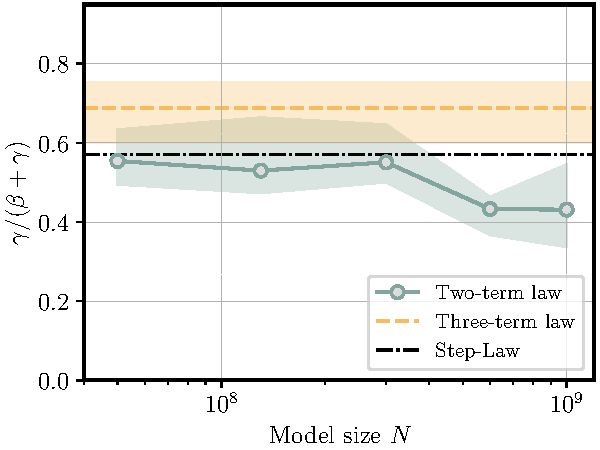
\includegraphics[width=0.99\linewidth]{plots/bs_step_scaling_law/oellm/optimal_batch_size_coefficient.pdf}
    \end{subfigure}
    %
    \begin{subfigure}[b]{0.49\columnwidth}
        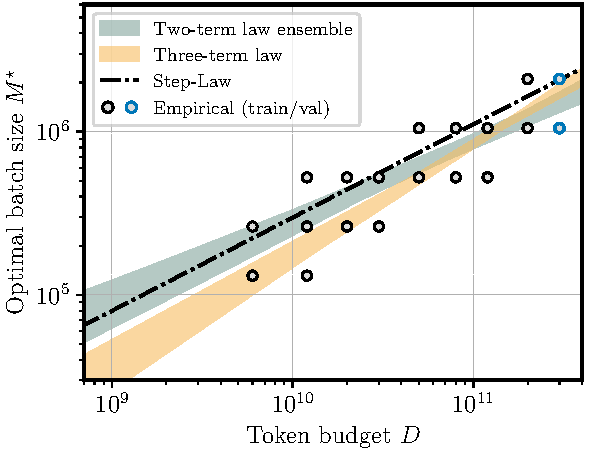
\includegraphics[width=0.99\linewidth]{plots/bs_step_scaling_law/oellm/optimal_batch_size_scaling.pdf}
    \end{subfigure}
    \caption{Same as \cref{fig:scaling-law-comparison-li}, but for \oellm{} dataset.}
    \label{fig:scaling-law-comparison-oellm}
\end{figure}
%
\begin{figure}[H]
    \centering
    \begin{subfigure}[b]{0.49\columnwidth}
        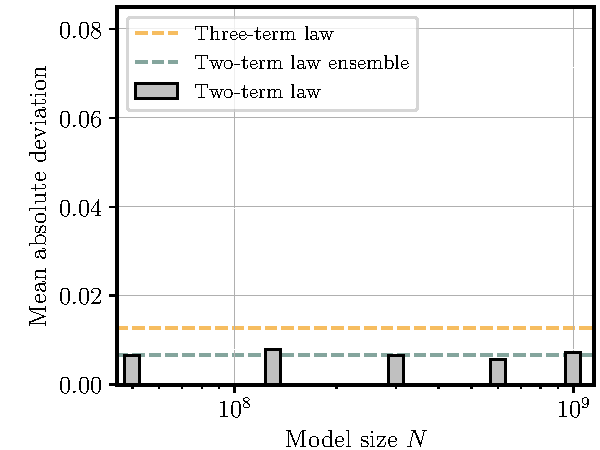
\includegraphics[width=0.99\linewidth]{plots/bs_step_scaling_law/oellm/mad_comparison_train.pdf}
    \end{subfigure}
    %
    \begin{subfigure}[b]{0.49\columnwidth}
        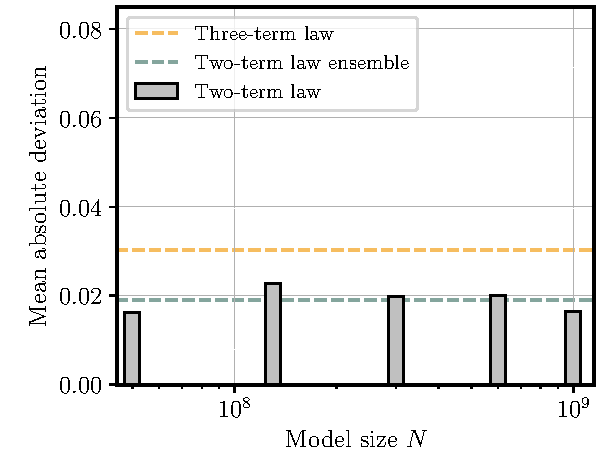
\includegraphics[width=0.99\linewidth]{plots/bs_step_scaling_law/oellm/mad_comparison_val.pdf}
    \end{subfigure}
    %
    \caption{Same as \cref{fig:mad-comparison-li}, but for \oellm{} dataset. \textbf{(Left)} Training set, \textbf{(right)} validation set.}
    \label{fig:mad-comparison-oellm}
\end{figure}
%


%%%%%%%%%%%%%%%%%%%%%%%%%%%%%%%%%%%%%%%%%%%%%%%%%%%%%%%
%
\subsection{Ablation on Value of $\delta$}\label{sec:app:ablation-delta}
%
When fitting the standard Chinchilla form \eqref{eqn:scaling-law} to the \li{} dataset with $\delta = 10^{-3}$, we observe that the variance in the parameter estimates appears to be unbalanced; this is likely due to the rather small range of $N$ in the dataset, which has been reported to cause issues for fitting scaling laws \citep{Li2025a}. We find that using $\delta = 10^{-5}$ fixes this. Hence, we perform an ablation with $\delta=10^{-5}$ for the two-term and three-term scaling laws, to check whether the value of $\delta$ impacts also the fit of those laws.

Below we show the results of \cref{sec:experiments:compare-2tl-3tl}, but using $\delta=10^{-5}$ instead of $\delta=10^{-3}$. In short, for \tttl{} we observe almost identical results, albeit with slightly higher variance for the scaling of $M^\star$. For \ttl{}, we observe a slightly worse MAD when using $\delta=10^{-5}$, as well as higher variance for the coefficients $(\gamma, \beta)$ as well as the scaling of $M^\star$.

Overall, the choice of $\delta$ does not have big impact on the conclusion of \cref{sec:experiments:compare-2tl-3tl}, with $\delta=10^{-3}$ being slightly preferable.
%
%
\begin{figure}[H]
    \centering
    \begin{subfigure}[b]{0.49\columnwidth}
        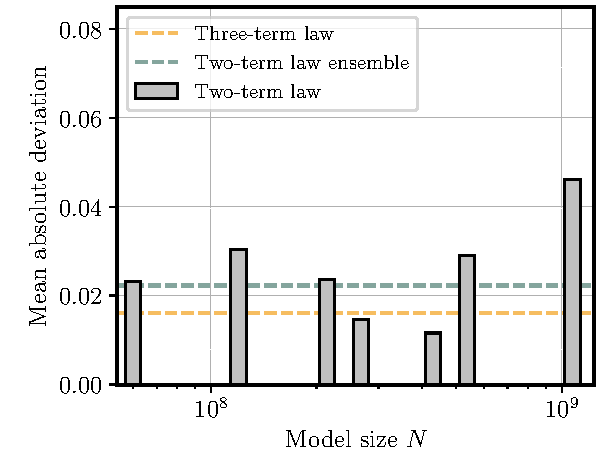
\includegraphics[width=0.99\linewidth]{plots/bs_step_scaling_law/li/ablations/delta/mad_comparison_train.pdf}
    \end{subfigure}
    %
    \begin{subfigure}[b]{0.49\columnwidth}
        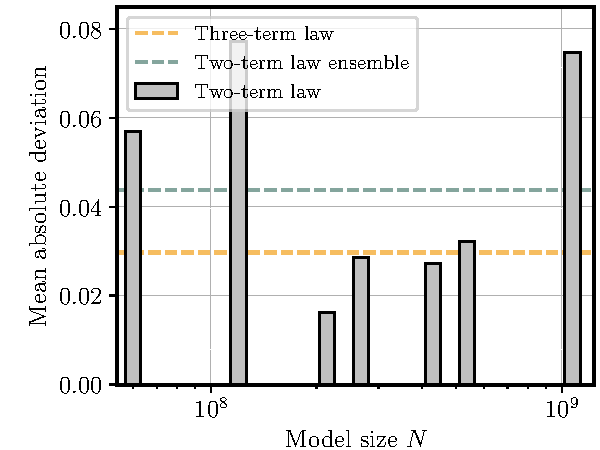
\includegraphics[width=0.99\linewidth]{plots/bs_step_scaling_law/li/ablations/delta/mad_comparison_val.pdf}
    \end{subfigure}
    %
    \caption{Same as \cref{fig:mad-comparison-li}, but with $\delta=10^{-5}$.}
    \label{fig:mad-comparison-li-ablate-delta}
\end{figure}
%
%
%
\begin{figure}[H]
    \centering
    \begin{subfigure}[b]{0.49\columnwidth}
        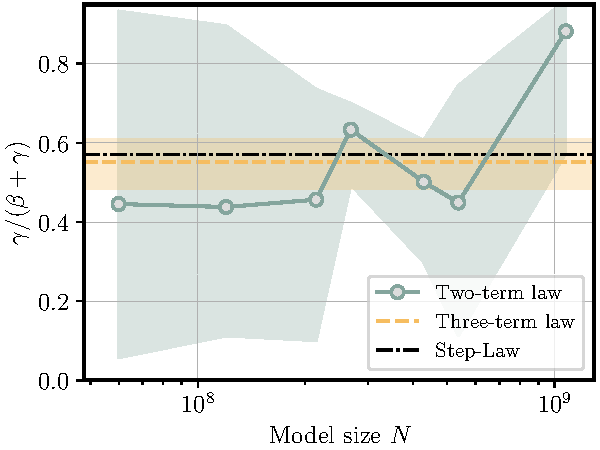
\includegraphics[width=0.99\linewidth]{plots/bs_step_scaling_law/li/ablations/delta/optimal_batch_size_coefficient.pdf}
    \end{subfigure}
    %
    \begin{subfigure}[b]{0.49\columnwidth}
        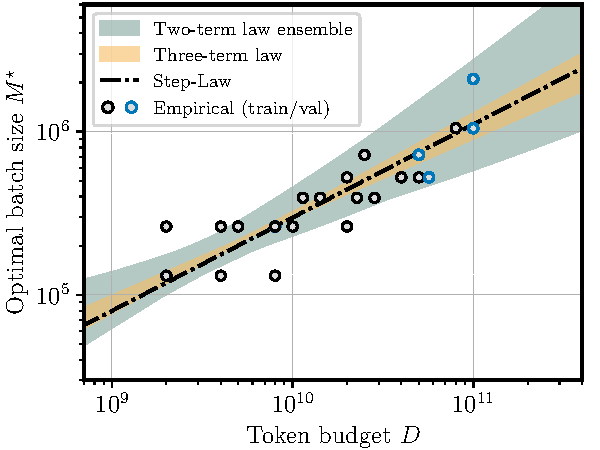
\includegraphics[width=0.99\linewidth]{plots/bs_step_scaling_law/li/ablations/delta/optimal_batch_size_scaling.pdf}
    \end{subfigure}
    \caption{Same as \cref{fig:scaling-law-comparison-li}, but with $\delta=10^{-5}$.}
    \label{fig:scaling-law-comparison-li-ablate-delta}
\end{figure}
%
\clearpage
%
\subsection{Additional Plots}\label{sec:app:plots}
%
%
\subsubsection{\li{} Dataset Overview}\label{sec:app:plots-li}
%
\begin{figure}[H]
    \centering
    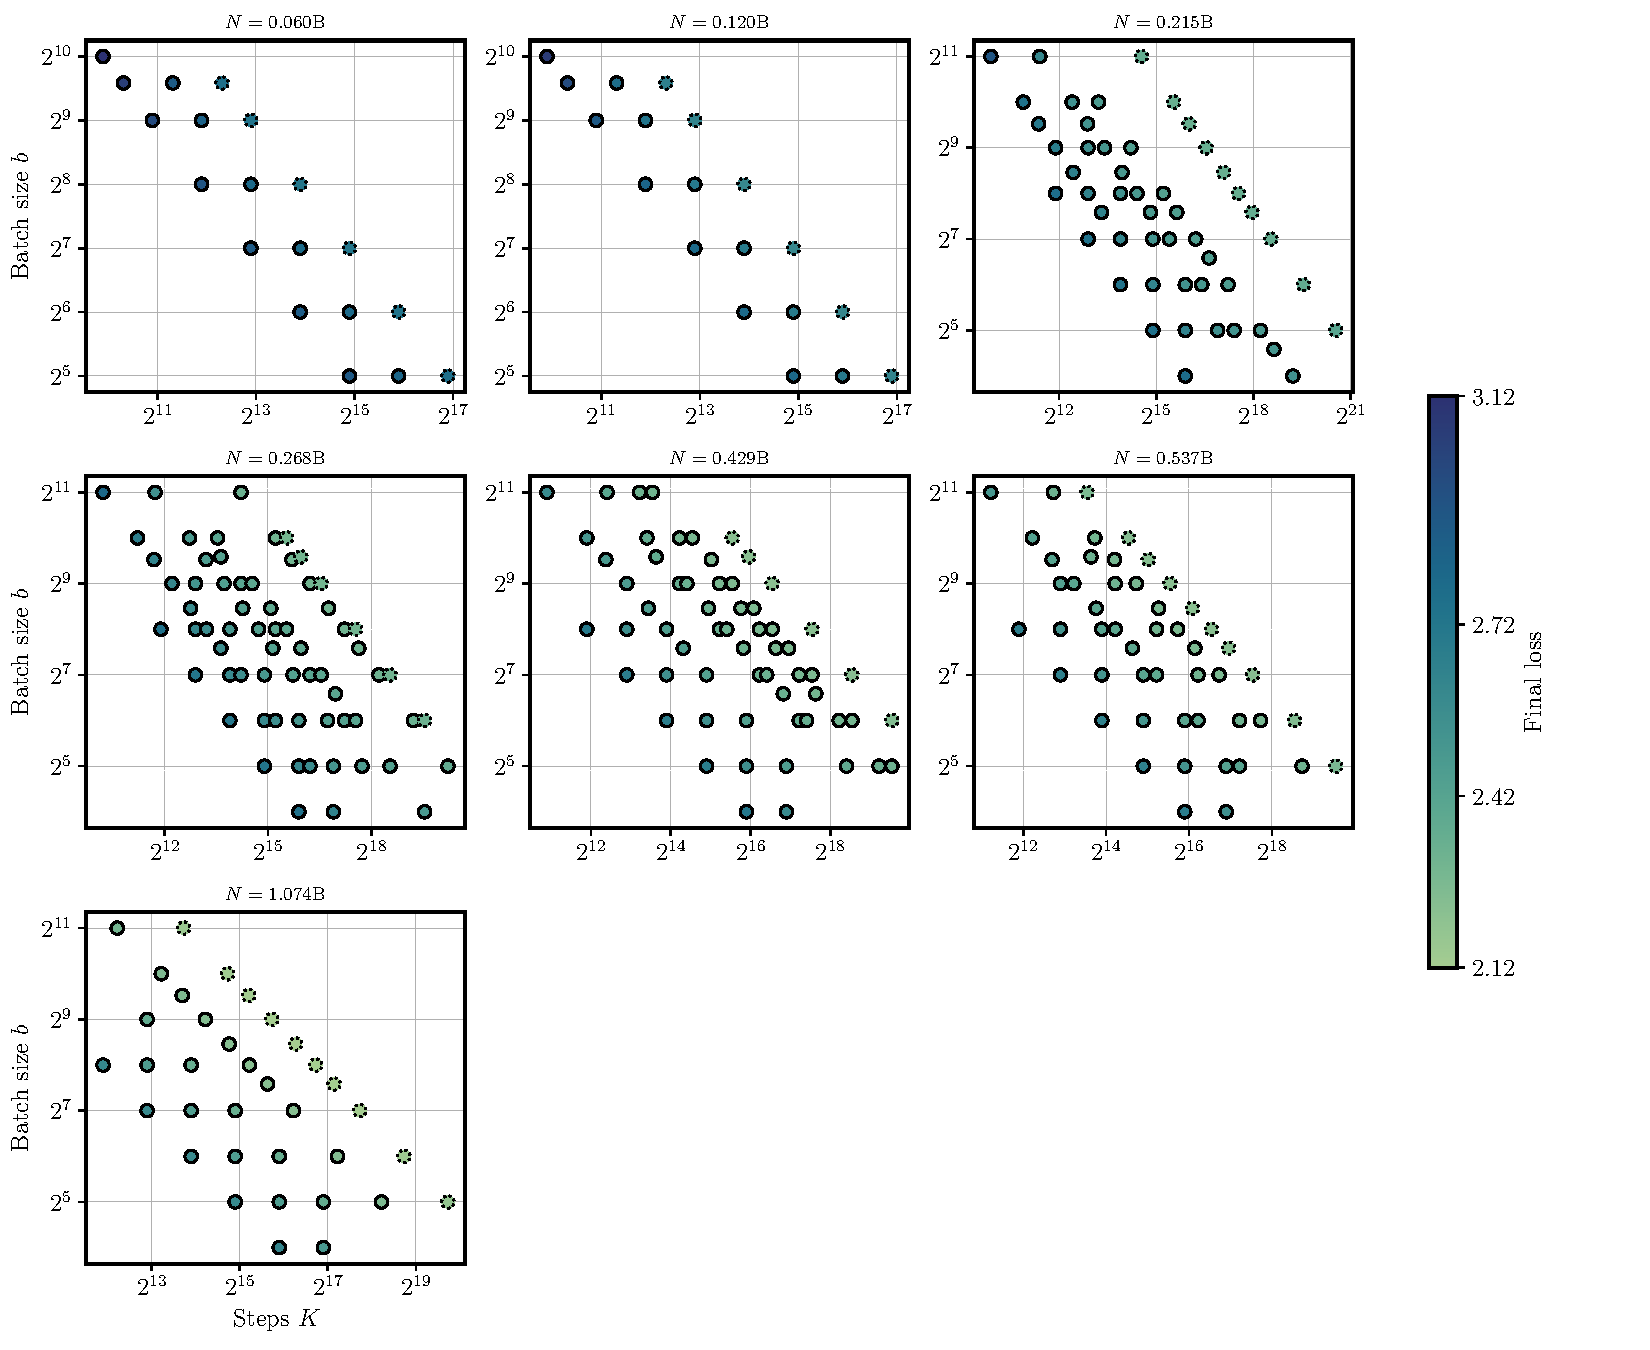
\includegraphics[width=0.99\linewidth]{plots/bs_step_scaling_law/li/runs_overview.pdf}
    \caption{Overview of the \li{} dataset used for fitting scaling laws. Dots with dashed border are part of the validation set.}
    \label{fig:data-overview-li}
\end{figure}
%
\clearpage
%
\begin{figure}[H]
    \centering
    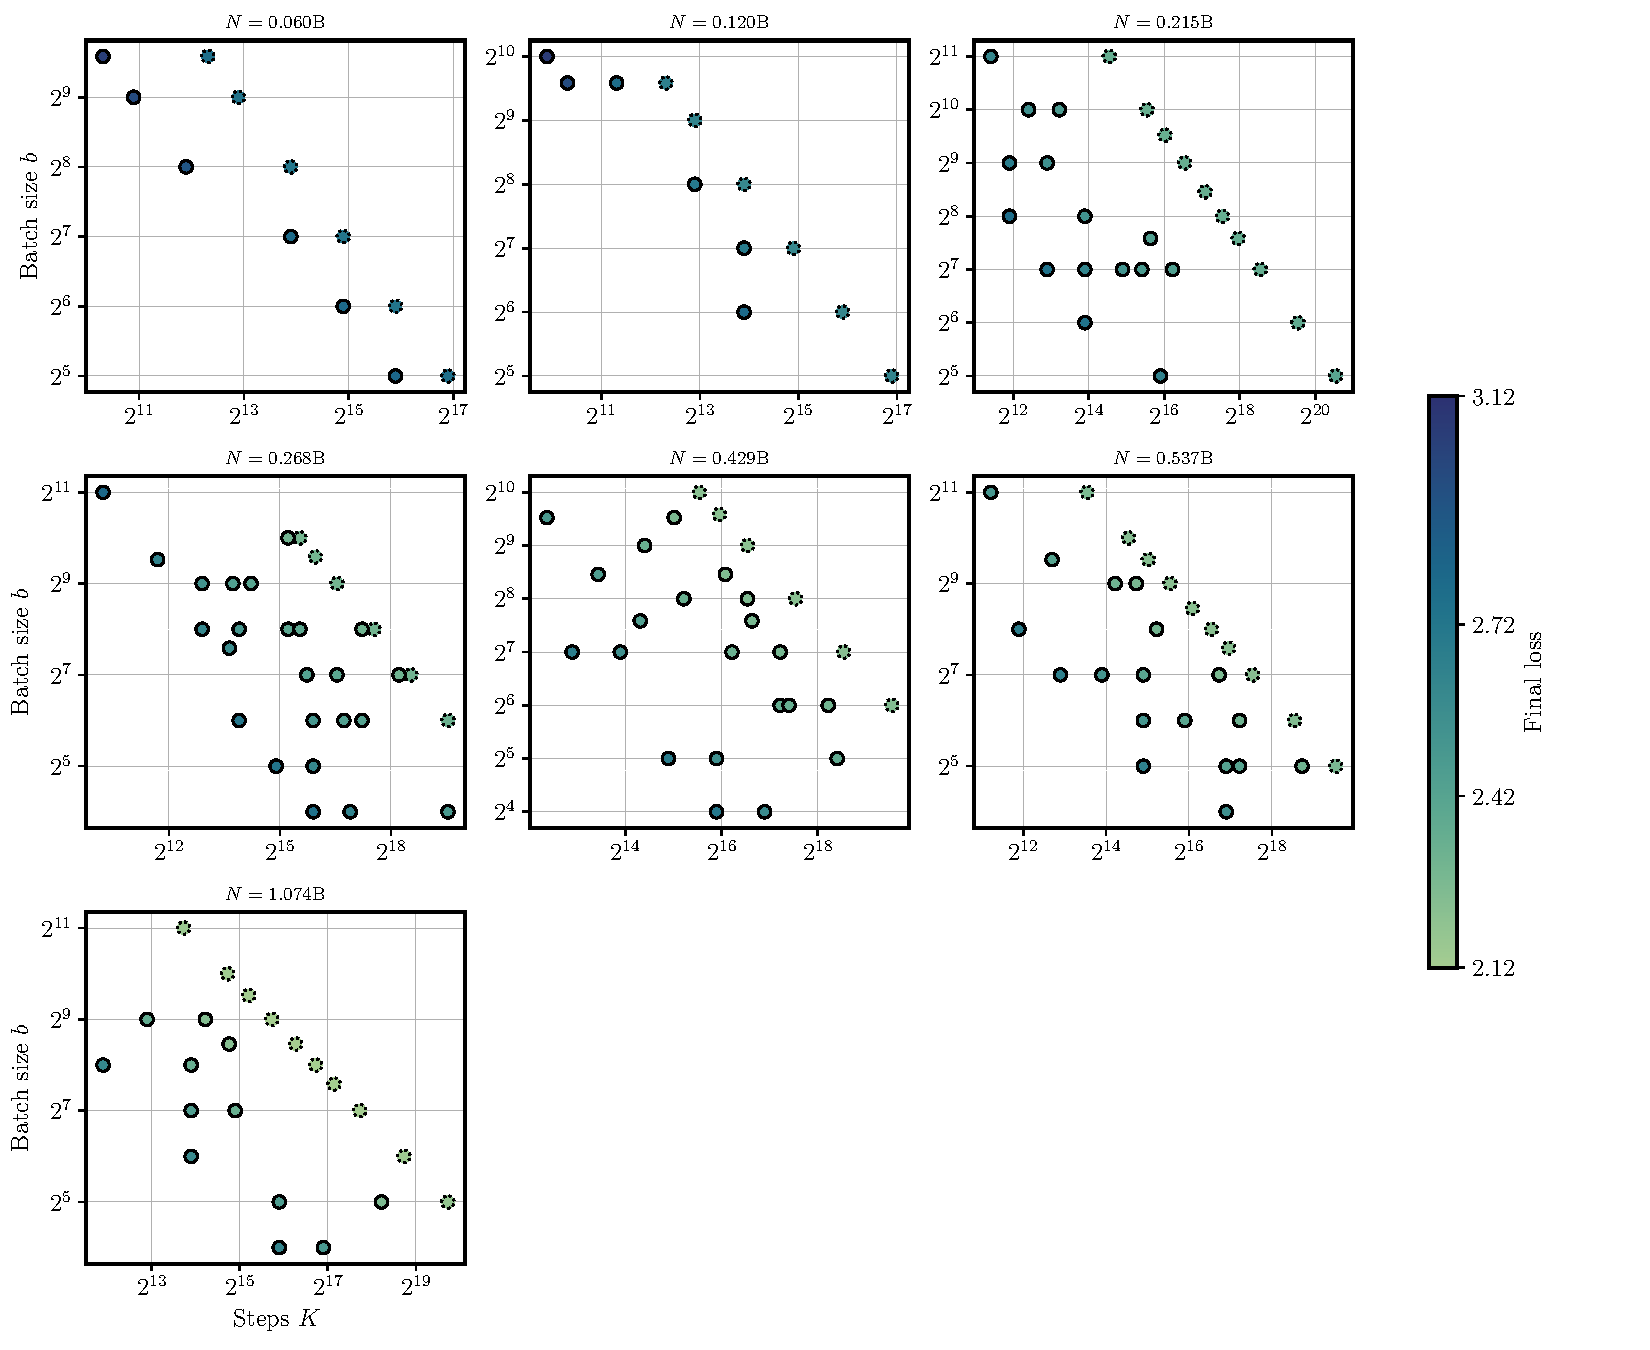
\includegraphics[width=0.99\linewidth]{plots/bs_step_scaling_law/li/ablations/mask3/runs_overview.pdf}
    \caption{Illustration of the reduced dataset used in \cref{sec:saving-compute}, with 3 batch size values $b$ per sweep. See also caption of \cref{fig:data-overview-li}; here, the difference is that for each value of $(N,D)$ we use only three different batch sizes (lying on a diagonal) for fitting, while the validation set remains the same as before.}
    \label{fig:data-overview-li-mask3}
\end{figure}
%
\clearpage
%
\begin{figure}[H]
    \centering
    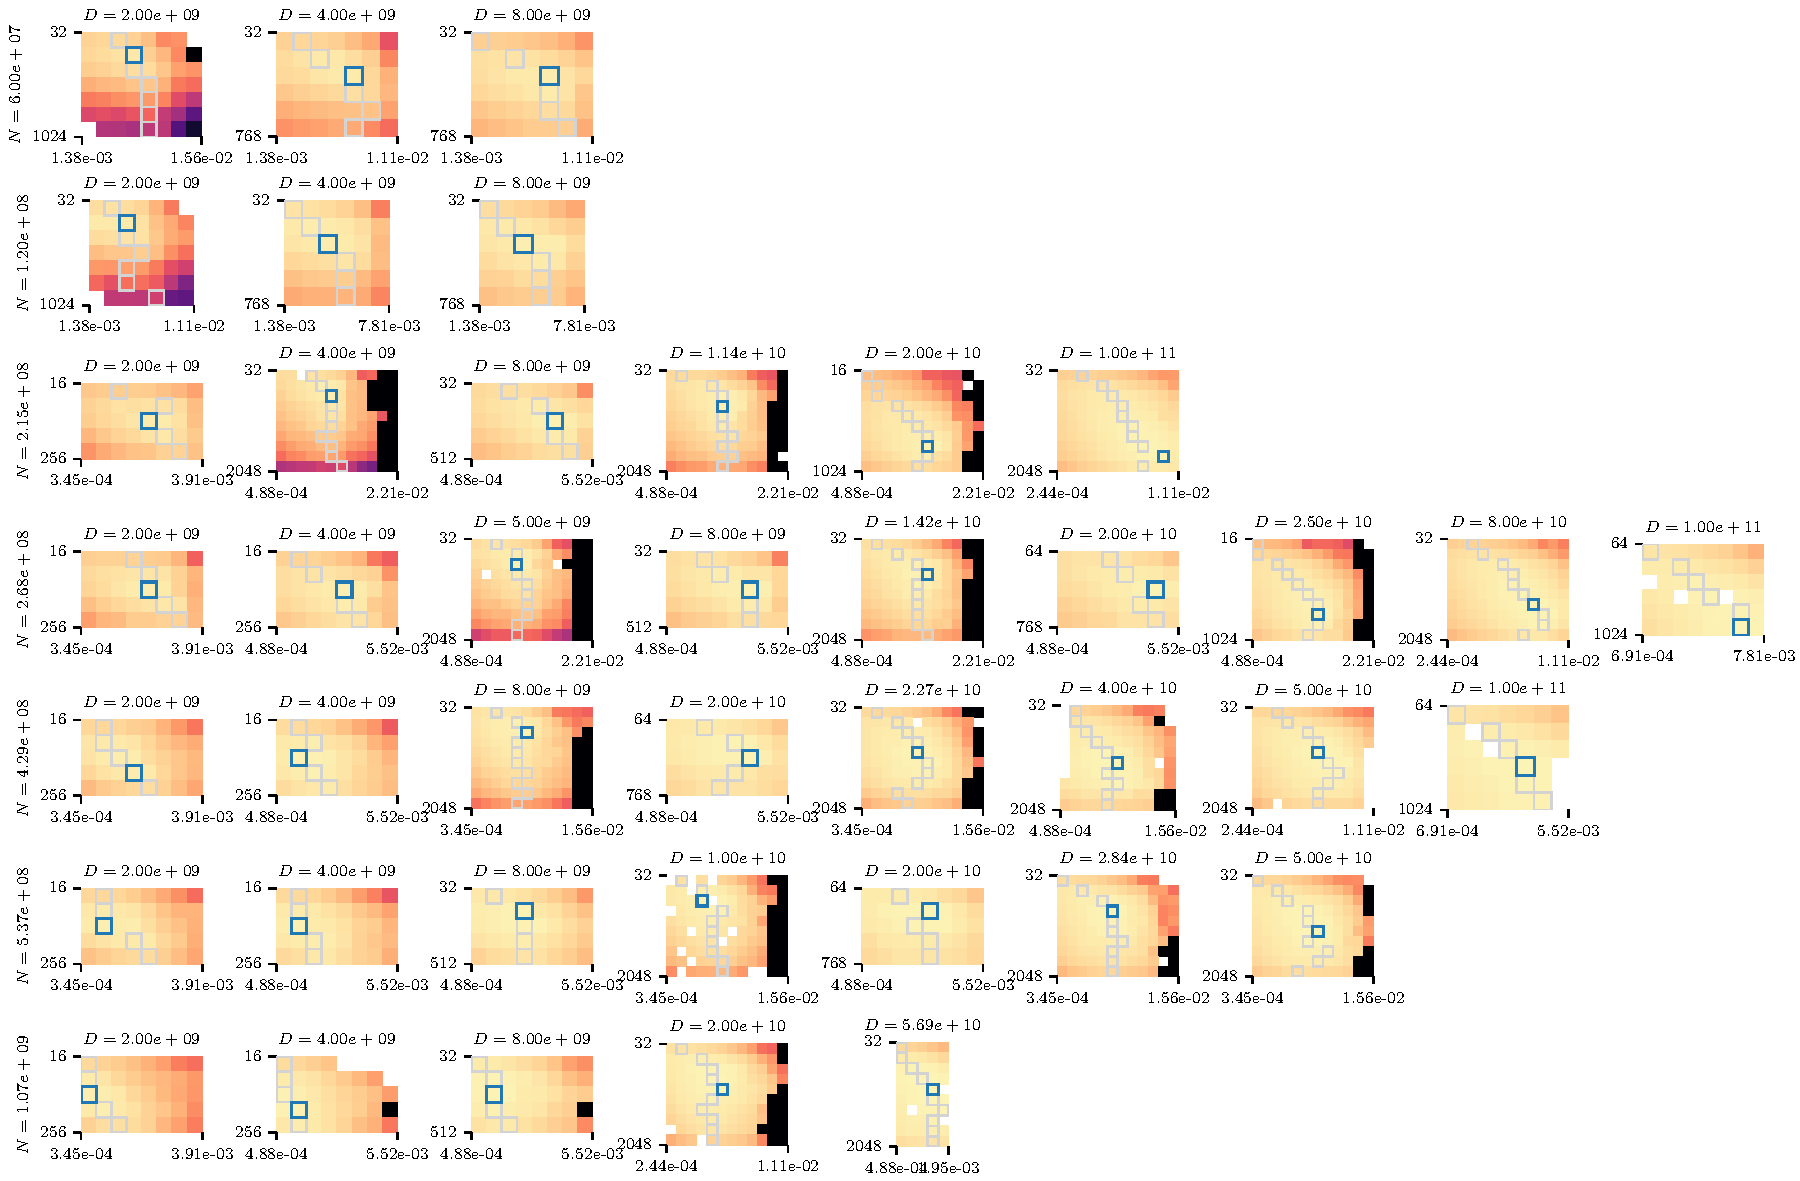
\includegraphics[width=0.99\linewidth]{plots/analysis/li/heatmaps.pdf}
    \caption{Overview of the full \li{} dataset (before learning-rate selection). Each heatmap represents the final loss over a grid of batch size $b$ ($y$-axis) and learning rate $\eta$ ($x$-axis) for a single combination of $(N,D)$. Blue squares mark the optimal combination of $(\eta, b)$, gray squares mark optimal learning rate for the given row of batch size. Note that most marked squares do not lie on the border, therefore indicating that the sweep is sufficiently extensive.}
    \label{fig:heatmaps-li}
\end{figure}

%%%%%%%%%%%%%%%%%%%%%%%%%%%%%%%%%%%%%%%%%%%%%%%%%%%%%%%%%%%%%%%%%%%%
%%%%%%%%%%%%%%%%%%%%%%%%%%%%%%%%%%%%%%%%%%%%%%%%%%%%%%%%%%%%%%%%%%%%
%%%%%%%%%%%%%%%%%%%%%%%%%%%%%%%%%%%%%%%%%%%%%%%%%%%%%%%%%%%%%%%%%%%%


\subsubsection{Suboptimal Batch Size Scaling: \li{}}\label{sec:app:subopt-bs-li}
%
%
\begin{figure}[H]
    \centering
    %
    \begin{subfigure}[b]{0.49\columnwidth}
        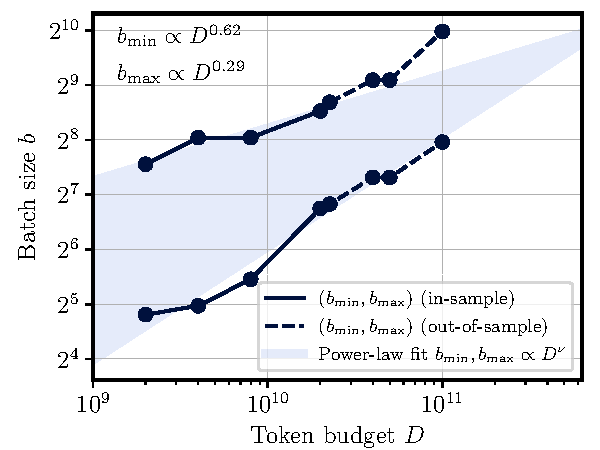
\includegraphics[width=0.99\linewidth]{plots/analysis_suboptimal_bs/li/suboptimal_bs_scaling_ms_429260800.pdf}
    \end{subfigure}
    %
    \begin{subfigure}[b]{0.49\columnwidth}
        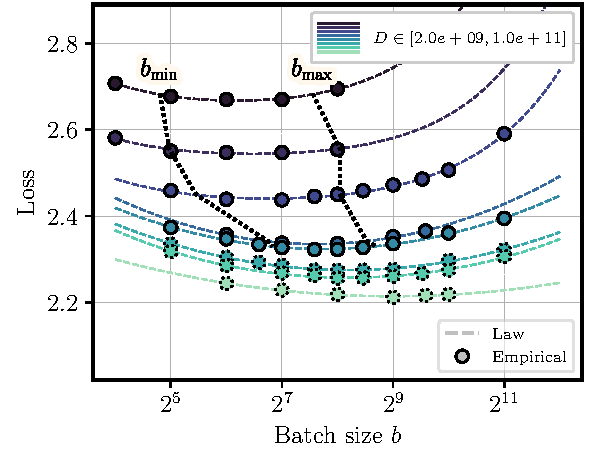
\includegraphics[width=0.99\linewidth]{plots/analysis_suboptimal_bs/li/bs_sweep_ms_429260800.pdf}
    \end{subfigure}
    %
    \caption{Same as \cref{fig:suboptimal-batch-size-two-stage}, but for $N=429$M.} 
    \label{fig:suboptimal-batch-size-two-stage-2}
\end{figure}
%
\begin{figure}[H]
    \centering
    %
    \begin{subfigure}[b]{0.49\columnwidth}
        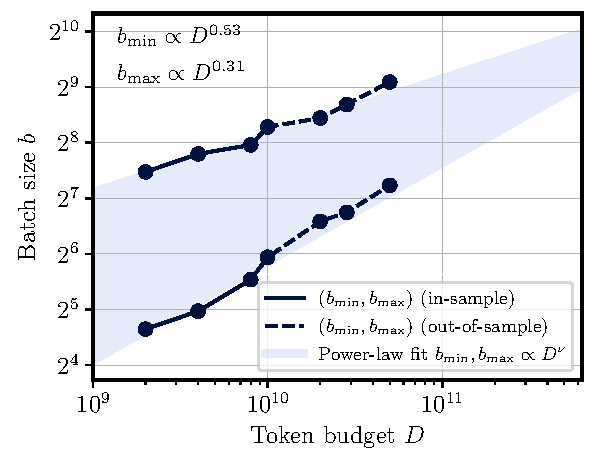
\includegraphics[width=0.99\linewidth]{plots/analysis_suboptimal_bs/li/suboptimal_bs_scaling_ms_536872960.pdf}
    \end{subfigure}
    %
    \begin{subfigure}[b]{0.49\columnwidth}
        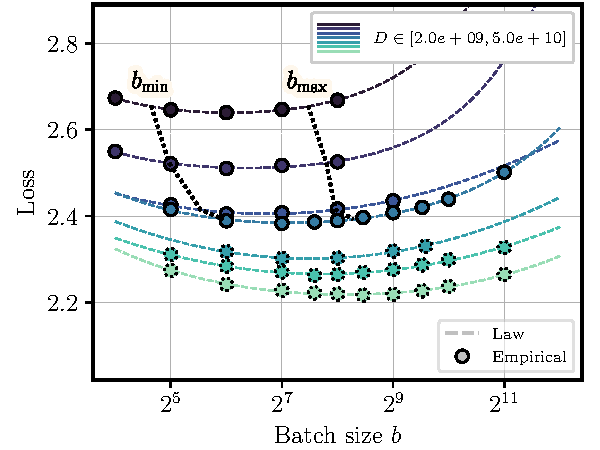
\includegraphics[width=0.99\linewidth]{plots/analysis_suboptimal_bs/li/bs_sweep_ms_536872960.pdf}
    \end{subfigure}
    %
    \caption{Same as \cref{fig:suboptimal-batch-size-two-stage}, but for $N=537$M.} 
    \label{fig:suboptimal-batch-size-two-stage-3}
\end{figure}
%
%
\subsubsection{Suboptimal Batch Size Scaling: \oellm{}}\label{sec:app:subopt-bs-oellm}
%
\begin{figure}[H]
    \centering
    %
    \begin{subfigure}[b]{0.49\columnwidth}
        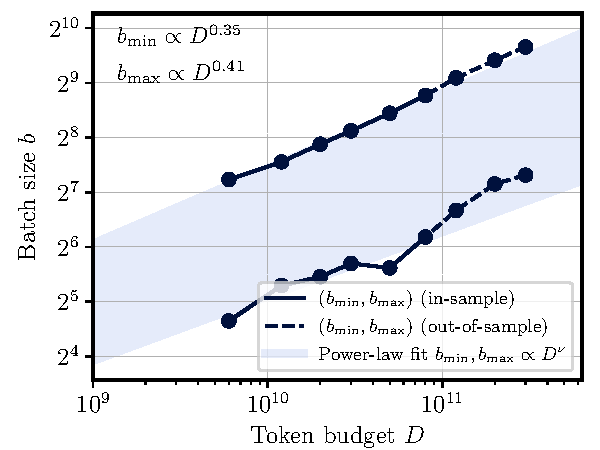
\includegraphics[width=0.99\linewidth]{plots/analysis_suboptimal_bs/oellm/suboptimal_bs_scaling_ms_300000000.pdf}
    \end{subfigure}
    %
    \begin{subfigure}[b]{0.49\columnwidth}
        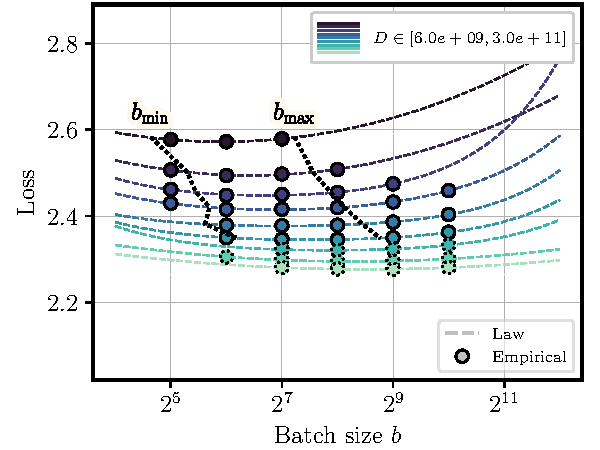
\includegraphics[width=0.99\linewidth]{plots/analysis_suboptimal_bs/oellm/bs_sweep_ms_300000000.pdf}
    \end{subfigure}
    %
    \caption{Same as \cref{fig:suboptimal-batch-size-two-stage}, but for \oellm{} dataset with $N=300$M.} 
    \label{fig:suboptimal-batch-size-two-stage-oellm}
\end{figure}
%
%
\begin{figure}[H]
    \centering
    %
    \begin{subfigure}[b]{0.49\columnwidth}
        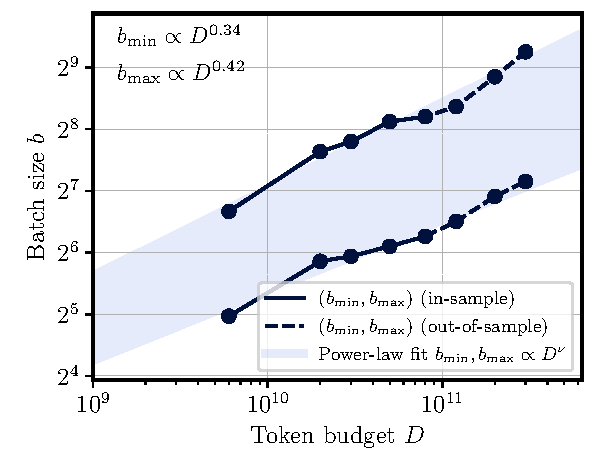
\includegraphics[width=0.99\linewidth]{plots/analysis_suboptimal_bs/oellm/suboptimal_bs_scaling_ms_1000000000.pdf}
    \end{subfigure}
    %
    \begin{subfigure}[b]{0.49\columnwidth}
        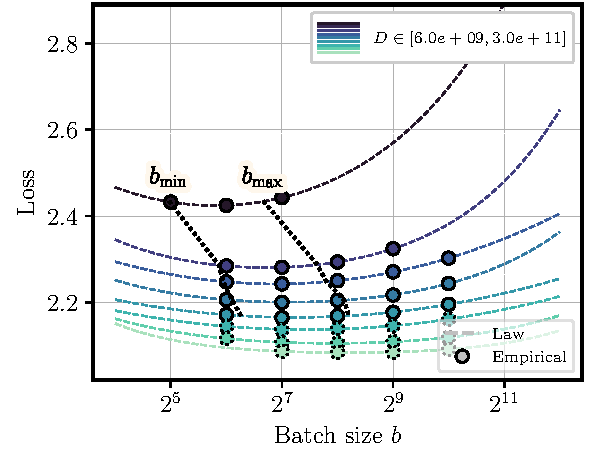
\includegraphics[width=0.99\linewidth]{plots/analysis_suboptimal_bs/oellm/bs_sweep_ms_1000000000.pdf}
    \end{subfigure}
    %
    \caption{Same as \cref{fig:suboptimal-batch-size-two-stage}, but for \oellm{} dataset with $N=1$B.} 
    \label{fig:suboptimal-batch-size-two-stage-oellm-2}
\end{figure}
%
\subsubsection{Reduced Dataset Fit for \oellm{}}\label{sec:app:reduced-fit-oellm}
%
%
\begin{figure}[H]
    \centering
    %
    \begin{subfigure}[b]{0.49\columnwidth}
        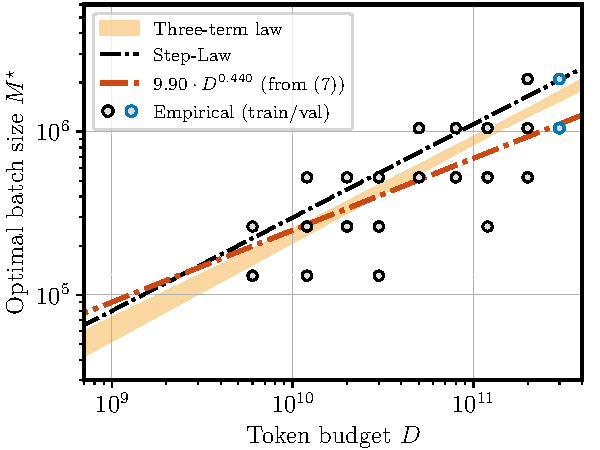
\includegraphics[width=0.99\linewidth]{plots/bs_step_scaling_law/oellm/ablations/mask3/optimal_batch_size_scaling.pdf}
        \caption{Dataset reduced to 63\%}
    \end{subfigure}
    %
    \begin{subfigure}[b]{0.49\columnwidth}
        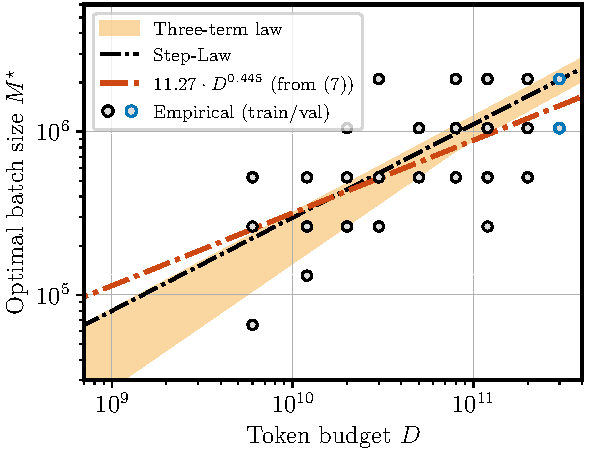
\includegraphics[width=0.99\linewidth]{plots/bs_step_scaling_law/oellm/ablations/mask2/optimal_batch_size_scaling.pdf}
        \caption{Dataset reduced to 42\%}
    \end{subfigure}
    %
    \caption{Same as \cref{fig:masked-optimal-bs-scaling}, but for \oellm{} dataset. Fitting on a reduced dataset, with only 3 values of $b$ per sweep \textbf{(left)} and 2 values \textbf{(right)}.
    } 
    \label{fig:masked-optimal-bs-scaling-oellm}
\end{figure}
%%%%%%%%%%%%%%%%%%%%%%%%%%%%%%%%%%%%%%%%%%%%%%%%%%%%%%%%%%%%%%%%%%
%%%%%%%%%%%%%%%%%%%%%%%%%%%%%%%%%%%%%%%%%%%%%%%%%%%%%%%%%%%%%%%%%%%%

